%\documentclass[
  bibliography=totoc,     % Literatur im Inhaltsverzeichnis
  captions=tableheading,  % Tabellenüberschriften
  titlepage=firstiscover, % Titelseite ist Deckblatt
]{scrartcl}

% Paket float verbessern
\usepackage{scrhack}

% Warnung, falls nochmal kompiliert werden muss
\usepackage[aux]{rerunfilecheck}

% unverzichtbare Mathe-Befehle
\usepackage{amsmath}
% viele Mathe-Symbole
\usepackage{amssymb}
% Erweiterungen für amsmath
\usepackage{mathtools}

% Fonteinstellungen
\usepackage{fontspec}
% Latin Modern Fonts werden automatisch geladen
% Alternativ zum Beispiel:
%\setromanfont{Libertinus Serif}
%\setsansfont{Libertinus Sans}
%\setmonofont{Libertinus Mono}

% Wenn man andere Schriftarten gesetzt hat,
% sollte man das Seiten-Layout neu berechnen lassen
\recalctypearea{}

% deutsche Spracheinstellungen
\usepackage[ngerman]{babel}


\usepackage[
  math-style=ISO,    % ┐
  bold-style=ISO,    % │
  sans-style=italic, % │ ISO-Standard folgen
  nabla=upright,     % │
  partial=upright,   % │
  mathrm=sym,        % ┘
  warnings-off={           % ┐
    mathtools-colon,       % │ unnötige Warnungen ausschalten
    mathtools-overbracket, % │
  },                       % ┘
]{unicode-math}

% traditionelle Fonts für Mathematik
\setmathfont{Latin Modern Math}
% Alternativ zum Beispiel:
%\setmathfont{Libertinus Math}

\setmathfont{XITS Math}[range={scr, bfscr}]
\setmathfont{XITS Math}[range={cal, bfcal}, StylisticSet=1]

% Zahlen und Einheiten
\usepackage[
  locale=DE,                   % deutsche Einstellungen
  separate-uncertainty=true,   % immer Unsicherheit mit \pm
  per-mode=symbol-or-fraction, % / in inline math, fraction in display math
]{siunitx}

% chemische Formeln
\usepackage[
  version=4,
  math-greek=default, % ┐ mit unicode-math zusammenarbeiten
  text-greek=default, % ┘
]{mhchem}

% richtige Anführungszeichen
\usepackage[autostyle]{csquotes}

% schöne Brüche im Text
\usepackage{xfrac}

% Standardplatzierung für Floats einstellen
\usepackage{float}
\floatplacement{figure}{htbp}
\floatplacement{table}{htbp}

% Floats innerhalb einer Section halten
\usepackage[
  section, % Floats innerhalb der Section halten
  below,   % unterhalb der Section aber auf der selben Seite ist ok
]{placeins}

% Seite drehen für breite Tabellen: landscape Umgebung
\usepackage{pdflscape}

% Captions schöner machen.
\usepackage[
  labelfont=bf,        % Tabelle x: Abbildung y: ist jetzt fett
  font=small,          % Schrift etwas kleiner als Dokument
  width=0.9\textwidth, % maximale Breite einer Caption schmaler
]{caption}
% subfigure, subtable, subref
\usepackage{subcaption}

% Grafiken können eingebunden werden
\usepackage{graphicx}

% schöne Tabellen
\usepackage{tabularray}
\UseTblrLibrary{booktabs, siunitx}

% Verbesserungen am Schriftbild
\usepackage{microtype}

% Literaturverzeichnis
\usepackage[
  backend=biber,
]{biblatex}
% Quellendatenbank
\addbibresource{lit.bib}
\addbibresource{programme.bib}

% Hyperlinks im Dokument
\usepackage[
  german,
  unicode,        % Unicode in PDF-Attributen erlauben
  pdfusetitle,    % Titel, Autoren und Datum als PDF-Attribute
  pdfcreator={},  % ┐ PDF-Attribute säubern
  pdfproducer={}, % ┘
]{hyperref}
% erweiterte Bookmarks im PDF
\usepackage{bookmark}

% Trennung von Wörtern mit Strichen
\usepackage[shortcuts]{extdash}

\author{%
  Vincent Wirsdörfer\\%
  \href{mailto:vincent.wirsdoerfer@udo.edu}{authorA@udo.edu}%
  \and%
  Joris Daus\\%
  \href{mailto:joris.daus@udo.edu}{authorB@udo.edu}%
}
\publishers{TU Dortmund – Fakultät Physik}


%\begin{document}
\section{Versuchsaufbau}
Das Herzstück des Versuches ist der Lock-In-Verstärker. Dieser kann eine Referenz- und Signalspannung erzeugen, erzeugte Spannungen mit 
Noise versehen und verstärken. Außerdem ist er dazu in der Lage Signale durch einen Phasenschieber zu verzögern und somit die Phase zu 
verändern. Verschiedene Filter können zur Bereinigung und Integration eines Signales verwendet werden.\\
\noindent
Das Experiment besteht aus zwei Versuchsaufbauten. 
Ein Versuchsaufbau dient dazu, den Einfluss eines Noisegenerators auf den Lock-In-Verstärker zu messen. Der zweite Aufbau testet 
den Lock-In-Verstärker unter real erzeugtem Noise.

\subsection{Künstlich generierter Noise}
\label{sec:kunstnoise}
Die Referenzspannung wird über einen Noisegenerator verrauscht und anschließend in einem Pre-Amplifier verstärkt. Das verstärkte Signal 
wird dann in einem Bandpass von sehr tiefen und hohen Frequenzen bereinigt. Anschließend geht dieses Signal dann in einen Detector.
Die Signalspannung geht durch einen Phasenschieber in den Lock-In-Verstärker. Das Ausgangssignal des Lock-In-Verstärkers wird ein digitales 
Oszilloskop eingespeist. So entsteht die folgende Schaltung.

\begin{figure}[H]
    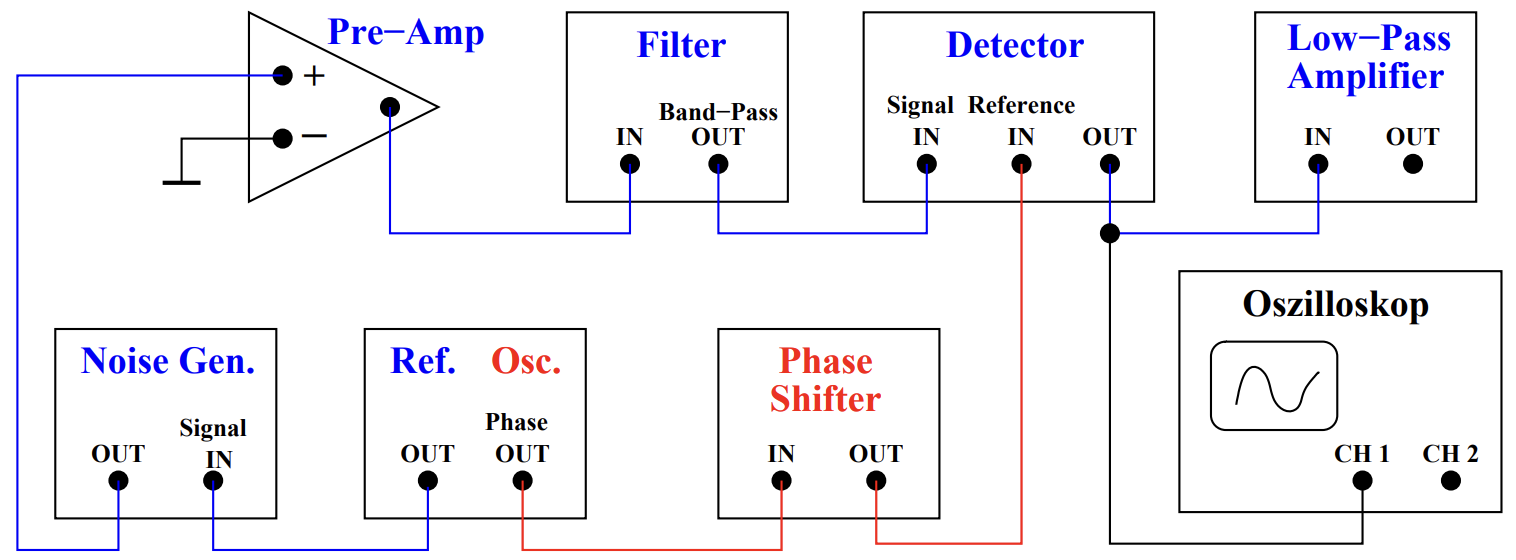
\includegraphics[width=\textwidth]{./content/Schaltung_kunstliche.png}
    \caption{Schaltung des Lock-In-Verstärkers mit künstlich generiertem Noise \cite{Versuchsanleitung_v303}}
    \label{fig:kunstnoise}
\end{figure}

\subsection{Noise durch Photodiode}
\noindent
Bei diesem Experimentaufbau wurde der Noisegenerator aus \autoref{sec:kunstnoise} durch eine LED mit Photodiode ausgetauscht. So ergibt sich 
die Schaltung \ref{fig:photonoise}

\begin{figure}[H]
    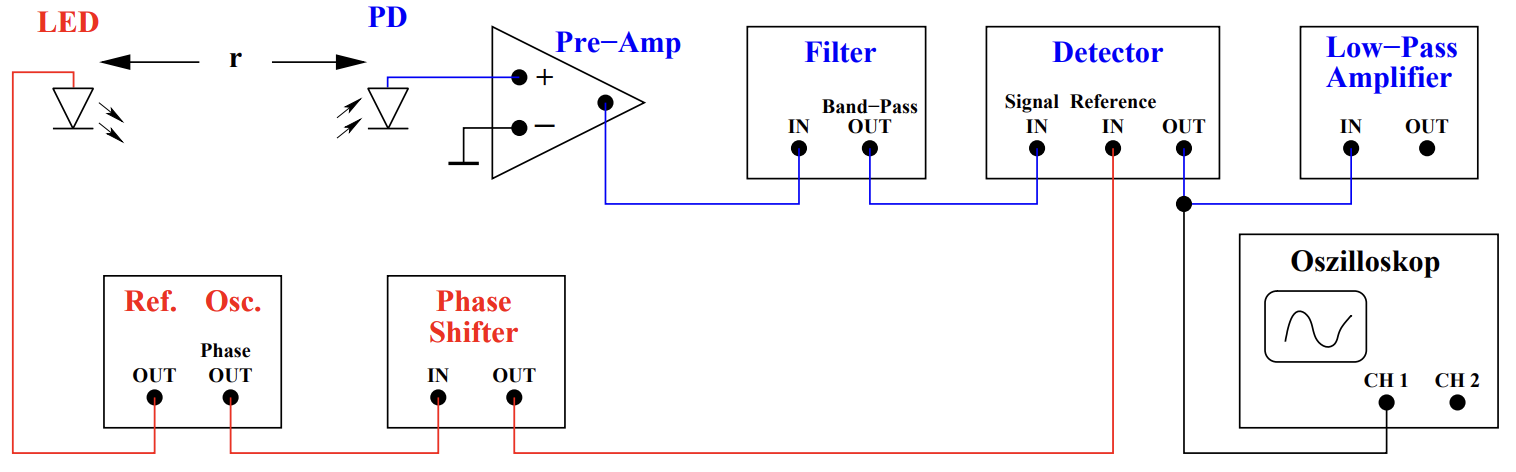
\includegraphics[width=\textwidth]{./content/Schaltung_Photodiode.png}
    \caption{Schaltung des Lock-In-Verstärkers mit Noise durch Photodiode \cite{Versuchsanleitung_v303}}
    \label{fig:photonoise}
\end{figure}

\noindent
Der Photodetektor ist auf einer Schiene montiert, sodass der Abstand $r$ aus \autoref{fig:photonoise} variiert werden kann.
Außerdem ist zu erwähnen, dass der Output an einem Integrator (also einem Tiefpass) angeschlossen ist, sodass das Signal über eine 
gewisse Zeitspanne integriert wird.


\section{Versuchsdurchführung}
Zunächst wird der Versuch mit dem Noisegenerator durchgeführt. Anschließend wird der Noise durch den Aufbau mit der Photidiode erzeugt.

\subsection{Künstlich generierter Noise}
\label{sec:durchf_kunst}
Es werden zwei Messreihen zur Überprüfung von Gleichung \eqref{eqn:U_out} aufgenommen. Zu Beginn wird der Noisegenerator auf \emph{OFF} gestellt.
Die Signalspannung ist sinusförmig und geht ungestört in den Lock-In-Verstärker. Dort wird sie mit der Referenzspannung, die vorher den 
Phasenschieber durchläuft gemischt. Die am Verstärker entstehende Spannung wird gegen die am Phasenschieber eingestellte Phase gemessen.
Anschließend wird der Noisegenerator eingeschaltet und somit die Signalspannung verunreinigt. Nun wird wieder die Spannung gegen die eingestellte 
Phase gemessen.

\subsection{Noise durch Photodiode}
In Experimentteil wird die Signalspannung an eine LED angeschlossen. Die LED wird mit der angeschlossenen Frequenz der Signalspannung an- und 
ausgeschaltet. Dieses Oszillieren wird von dem Photodetektor detektiert und in eine Spannung umgwewandelt. Diese Spannung ist aufgrund von dem 
Umgebungslicht und Streuungen von der ursprünglichen Spannung verschieden und somit verunreinigt. Sie geht somit als Signalspannung in den 
Lock-In-Verstärker. Die Referenzspannung wird wie im anderen Experimentaufbau über einen Phasenschieber in den Verstärker eingespeist. 
Der Ausgang des Verstärker ist an einem Tiefpassfilter zum integrieren angeschlossen. Es wird eine bestimmtes Zeitfenster eingestellt, über das 
integriert wird. Dieses wird während des versuches nicht verändert.\\
\noindent Nun wird der Photodetektor auf der Schiene nach hinten verschoben und nach jeder Verschiebung das integrierte Signal gemessen.  



\section{Messwerte}
Im folgenden werden die Messwerte beider Experimentaufbauten getrennt voneinander aufgelistet.

\subsection{Künstlich generierter Noise}
Die Messung des nicht verauschten Signales ergibt folgende Messdaten:

\begin{table}[H]
    \centering
    \sisetup{per-mode=reciprocal}
    \begin{tblr}{colspec = {S[table-format=3] S[table-format=1.2]}, row{1} = {guard, mode=math}}
    \toprule
    \phi \mathbin{/} \unit{\degree} &
    U \mathbin{/} \unit{\volt} \\
    \midrule
    0   &   0.34 \\
    15  &   0.38 \\
    45  &   0.56 \\
    60  &   0.62 \\
    90  &   0.62 \\
    135 &   0.52 \\
    150 &   0.4  \\
    180 &   0.24 \\
    225 &   0.04 \\
    270 &   -0.04\\
    315 &   0.08 \\
    330 &   0.2  \\
    360 &   0.34 \\
    \end{tblr}
    \caption{Phasenverschiebung gegen Spannung ohne Verrauschung.}
    \label{tab:no_noise}
\end{table}

\noindent
Im Anschluss wurde die Messung wiederholt, jedoch wurde dabei die Signalspannung durch einen Noisegenerator geführt. So ergeben sich folgende 
Messdaten:

\begin{table}[H]
    \centering
    \sisetup{per-mode=reciprocal}
    \begin{tblr}{colspec = {S[table-format=3] S[table-format=1.1]}, row{1} = {guard, mode=math}}
    \toprule
    \phi \mathbin{/} \unit{\degree} &
    U \mathbin{/} \unit{\volt} \\
    \midrule
    0   &   0   \\
    15  &   0   \\
    45  &   0.3 \\
    60  &   0.6 \\
    90  &   1   \\
    135 &   1.5 \\
    150 &   1.7 \\
    180 &   1.6 \\
    210 &   1.6 \\
    225 &   1.4 \\
    315 &   0.2 \\
    330 &   0   \\
    360 &   0   \\
    \end{tblr}
    \caption{Phasenverschiebung gegen Spannung mit Verrauschung.}
    \label{tab:mit_noise}
\end{table}


\subsection{Noise durch Photodiode}
Nun werden die Messdaten für den zweiten Experimentaufbau dargelegt. Dabei wird der Abstand $A$ des Photodetektors zur LED gegen die 
integrierte Spannung $U$ aufgetragen:

\begin{table}[H]
    \centering
    \sisetup{per-mode=reciprocal}
    \begin{tblr}{colspec = {S[table-format=2] S[table-format=1.4]}, row{1} = {guard, mode=math}}
    \toprule
    A \mathbin{/} \unit{\centi \meter} &
    U \mathbin{/} \unit{\volt} \\
    \midrule
    5   &   7.9     \\
    6   &   5.95    \\
    7   &   4.8     \\
    8   &   3.9     \\
    9   &   3.25    \\
    10  &   2.6     \\
    11  &   2.4     \\
    12  &   1.95    \\
    13  &   1.6     \\
    14  &   1.45    \\
    15  &   1.25    \\
    16  &   1.05    \\
    17  &   0.95    \\
    18  &   0.825   \\
    19  &   0.75    \\
    20  &   0.7     \\
    25  &   0.4375  \\
    30  &   0.2775  \\
    35  &   0.1875  \\
    40  &   0.125   \\
    45  &   0.1275  \\
    50  &   0.0975  \\
    55  &   0.0775  \\
    60  &   0.065   \\
    65  &   0.0525  \\
    70  &   0.0475  \\
    75  &   0.04    \\
    80  &   0.035   \\
    85  &   0.03    \\
    90  &   0.025   \\
    \end{tblr}
    \caption{Abstand gegen die Spannung am Photodetektor.}
    \label{tab:photonoise}
\end{table}

\noindent
Die Spannung am Photodetektor fällt der Theorie nach schnell ab, weshalb für kleine Abstände die Messabstände geringer sind als für 
große Abstände.

%\end{document}

